\mysection{Méthodologie}
Cette section a comme but expliquer les méthodes utilisées pour faire chaque tâche des parties 2 a 4 du travail, décrits dans les sections \ref{Deuxième Partie - Mise en Main} a \ref{Quatrième Partie - Intégration}.

\newcommand{\powerfactory}{DIgSILENT PowerFactory}
\mysubsection{Deuxième Partie - Mise en Main}
Comme dit, le logiciel \powerfactory a été utilisé pour faire des simulations du réseau, donc une petit explication du réseau e du logiciel sera fait dans cette section.

\mysubsubsection{Sur le \powerfactory}
Le \powerfactory est un logiciel beaucoup utilisé dans le métier d'Énergie, par entreprises comme \gls{EDF}, \gls{Enedis} pour faire des simulations des réseau électriques, que les permettent de vérifier stabilité en cas de panne et surcharge ou sous-charge de parties du réseau, calculer coûts d'opération et même programmer autres changements futur du réseau. Quelques autres instituts comme L'\gls{IETR} et \gls{Polimi}, par exemple l'utilise pour ses thèmes des thèses et autres recherches.   

\begin{figure}[H]
	\begin{center}	
		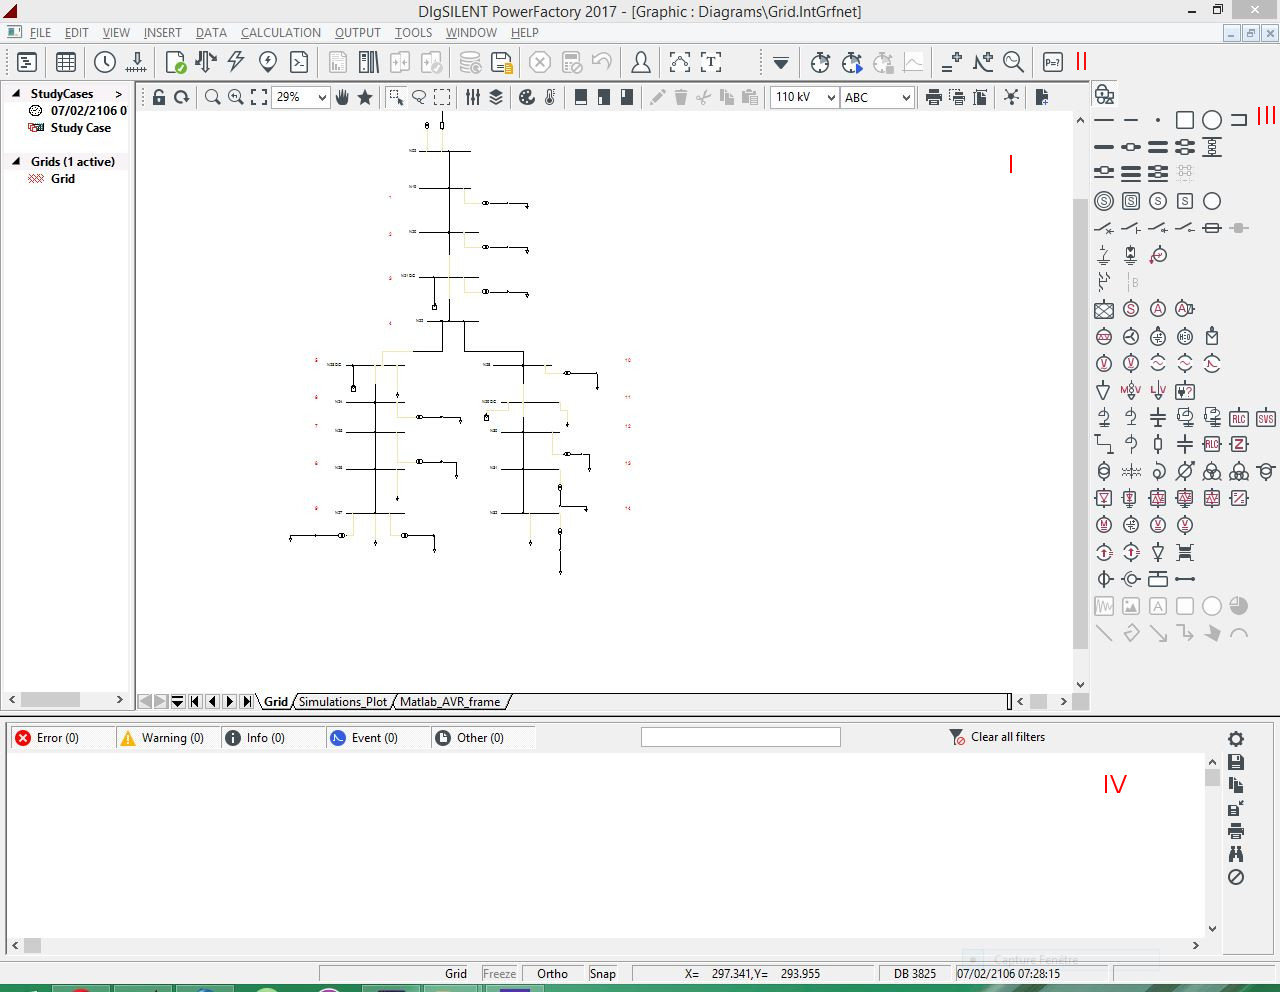
\includegraphics[width=\textwidth]{Methodologie/partie_2/gui_powerfactory_num.JPG}
		\caption{\gls{GUI} du \powerfactory.}
		\label{fig:gui_powerfactory}
	\end{center}
\end{figure}

\pagebreak
En peut voir dans la figure \ref{fig:gui_powerfactory} quelques panneaux basiques importants du \gls{GUI} du \powerfactory

\begin{enumerate}[I]
	\item Panneau Graphique\\ Où les diagrammes sont affichés, tant réseaux quant graphiques.
	\item Panneau des Outil\\ Où sont concentrés les outils du programme, pour modifier l'affichage, donnant une couleur différente par chaque bus par exemple; faire des diverses types de simulation,  de Court-circuit, calculs de flux de charge simulation \gls{RMS} et \gls{EMT}, etc.
	\item Panneau de Dessin\\ Outils pour dessiner des éléments du réseau, comme bus, transformateur, charge etc
	\item Panneau de Sortie\\ Où sont montrés les résultats des calculs et simulations, les avertissement et les erreurs.
\end{enumerate}


\mysubsection{Sur le réseau}
Comme était dit, la figure \ref{fig:Diagramme_du_reseaux} démontre le réseau utilisé. On peut voir que le réseau est formé pour 16 charges et 3 générateurs distribués, 12 transformateurs.
Dans le réseau original les générateurs étaient des machines synchrones mais elles ont été remplacé par des panneaux photovoltaïque, a fin de faire les réponses des tests plus vite, en vue de la dynamique des panneaux considérablement plus vite que des machines synchrones. 

\begin{table}[H]
	\captionsetup{justification=centering,margin=2cm}
	\caption{Générateurs Distribués du Réseau }
	\centering
	\begin{tabular}{m{1cm}m{1.5cm}m{1.5cm}}
		\hline
		GD&P[MW] nominal&P[MW] 1p.m.\\
		\hline\\
		GD4&3.2&2.056124\\
		GD5&5.5&4.94595\\
		GD6&5.5&3.245381\\
		\hline\\
	\end{tabular}
\end{table}	

\begin{table}[H]
	\captionsetup{justification=centering,margin=2cm}
	\caption{Transformateurs HV/MV }
	\centering
	\begin{tabular}{lc}
		\hline
		Model&40 MVA132/20\\
		\hline\\
		Puissance&50MVA\\
		Pertes Cuivre&176kW\\
		Tension de court-circuit Relative&15.5\%\\
		Taps&12\\
		Tension per Tap&1.5\%\\
		\hline\\
	\end{tabular}
\end{table}	

\begin{table}[H]
	\captionsetup{justification=centering,margin=2cm}
	\caption{Transformateurs MV/LV }
	\centering
	\begin{tabular}{lm{2cm}m{2cm}m{2cm}}
		\hline
		Modèle&0.25MVA 20kV/0.4&0.4MVA 20kV/0.4&0.63MVA 20kV/0.4\\
		\hline\\
		Puissance&250kVA&400kVA&630kVA\\
		Pertes Cuivre&2.6kW&3.7 kW&5.6kW\\
		Tension de court-circuit Relative&4\%&4\%&4\%\\
		Nombres de Transformateurs&1&6&4\\
		\hline\\
	\end{tabular}
\end{table}	

\newcommand{\trafoi}{40 MVA132/20}
\newcommand{\trafoii}{0.25MVA 20kV/0.4}
\newcommand{\trafoiii}{0.4MVA 20kV/0.4}
\newcommand{\trafoiv}{0.63MVA 20kV/0.4}
\begin{table}[H]
	\captionsetup{justification=centering,margin=2cm}
	\caption{Transformateurs}
	\centering
	\begin{tabular}{cc}
		\hline
		Nom&Modèle\\
		\hline\\
		TR AT/MT&\trafoi\\
		TR 2.19&\trafoiv\\
		TR 2.20&\trafoiii\\
		TR 2.21&\trafoiii\\
		TR 2.24&\trafoiii\\
		TR 2.25&\trafoiii\\
		TR 2.27.1&\trafoiv\\
		TR 2.27.3&\trafoiv\\
		TR 2.28&\trafoii\\
		TR 2.30&\trafoiv\\
		TR 2.31&\trafoiii\\
		TR 2.32&\trafoiii\\
		\hline\\
	\end{tabular}
\end{table}	

\newcommand{\cablei}{ARG7H1RX 185mmq}
\newcommand{\cableii}{ARG7H1RX 70mmq}
\newcommand{\cableiii}{Aerea Cu 70mmq}

\begin{table}[H]
	\captionsetup{justification=centering,margin=2cm}
	\caption{Lignes}
	\centering
	\begin{tabular}{llccccc}
		\hline
		Nom&Genre&Section[$ mm^2 $]&R[$ \Omega/km $]&L[$ mH/km $]&C[$ \mu F/km $]\\
		\hline\\
		\cablei&Câble&185&0.2180&.0350&0.2900\\
		\cableii&Câble&70&0.5800&0.41&0.2100\\
		\cableiii&Aérien&70&0.2681&1.286&0.0090\\
		\hline\\
	\end{tabular}
\end{table}	


\begin{table}[H]
	\captionsetup{justification=centering,margin=2cm}
	\caption{Caractéristiques des Lignes}
	\centering
	\begin{tabular}{ccc}
		\hline
		Nom&Genre&Longueur[$ km $]\\
		\hline\\
		D2-02\_19&\cablei&3.6\\
		D2-19\_20	&\cablei&3.304\\
		D2-20\_21	&\cableiii&2.4\\
		D2-21\_22	&\cableiii&3.6\\
		D2-22\_23	&\cableiii&3\\
		D2-22\_28	&\cableii&2.4\\
		D2-23\_24	&\cableiii&3.08\\
		D2-24\_25	&\cableiii&1.65\\
		D2-25\_26	&\cableiii&1.8\\
		D2-26\_27	&\cableiii&2.2\\
		D2-28\_29	&\cableii&2.2\\
		D2-29\_30	&\cableii&2.4\\
		D2-30\_31	&\cableii&2.6\\
		D2-31\_32	&\cableii&2.7\\
		\hline\\
	\end{tabular}
\end{table}	

\begin{table}[H]
	\captionsetup{justification=centering,margin=2cm}
	\caption{Charges}
	\centering
	\begin{tabular}{cccc}
		\hline
		Nom&Genre&P[$ MW $]1p.m.&Q[$MVAR$]1p.m.\\
		\hline\\
		C 2-19 &LV&0.1894&0.1265088\\
		C 2-20 &LV&0.1147&0.0774413\\
		C 2-21 &LV&0.1155&0.0782289\\
		C 2-23&MV&0&0.1\\
		C 2-24 &LV&0.1094&0.0741473\\
		C 2-25 &LV&0.1450&0.0984401\\
		C 2-26&MV&0.3993&0.2049369\\
		C 2-27.1&LV&0.2471&0.1656134\\
		C 2-27.2& MV&.6083&0.2971269\\
		C 2-27.3& LV&0.2094&0.1407233\\
		C 2-28 &LV&0.1205&0.08741\\
		C 2-29 &MV&0.1561&0.0798601\\
		C 2-30 &LV&0.1934&0.1347733\\
		C 2-31 &LV&0.0934&0.0640347\\
		C 2-32.1 &LV&0.1333&0.0923274\\
		C 2-32.2 &MV&0.5634&0.2791258\\
		\hline\\
	\end{tabular}
\end{table}	

\mysection{Troisième Partie - Programmation}


\begin{figure}[H]
	\begin{center}	
		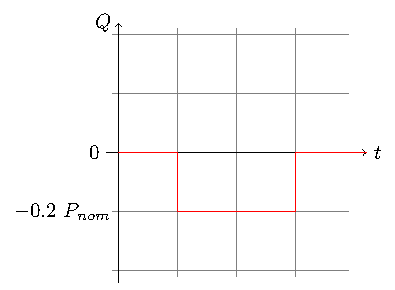
\includegraphics[width=8cm]{Methodologie/partie_3/gain_calc-generator2bus-test_1.pdf}
		\caption{Allure de la courbe utilisé pendant le Test 1}
		\label{fig:gaincalcgenerator2bustest1}
	\end{center}
\end{figure}

\begin{figure}[H]
	\begin{center}	
		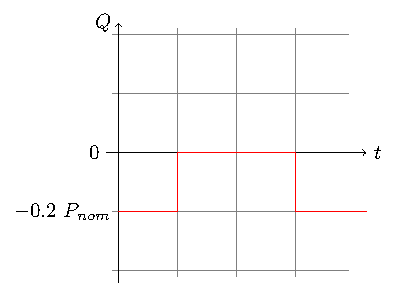
\includegraphics[width=8cm]{Methodologie/partie_3/gain_calc-generator2bus-test_2.pdf}
		\caption{Allure de la courbe utilisé pendant le Test 2}
		\label{fig:gaincalcgenerator2bustest2}
	\end{center}
\end{figure}



























